\section{Operations Research Model}

{\color{red} 
	
	Introduce proposed concepts in the Operations Research Model (OR model).
	
	The OR model is a combination of Steel Manufacturing Events Analysis and Flux Balance Analysis. The art form of this model is to structure a standard data format and a shared analysis logic that allows comparing the results from manufacturing data and simulation data.
	
	A brief introduction for Association Networks and FBA. 
	An explanation for generating a data structure with OR-modeling in the combination of those. More detailed information to be given in the Backgroud Information Section, guiding the readers who have knowledge of FBA and Association Network concepts to the Concept Implementation Section.
	
	Usage of linear programming and generating sets of synthetic data allow comparing the statistical characteristics of their association network with those created from the real-world data set from steel manufacturing.
	
}

\clearpage

\subsection{Steel Manufacturing Data Analysis}
\subsection*{Association Networks}
\addcontentsline{toc}{subsection}{Association Networks}%
{\color{red}Beyond a simple network graph representation of historical production data, the formation of association rules networks is an insightful graph-based framework combining the tools: association rules and complex networks, as Merten et al. (2020) performed in their article~\cite{MERTEN2020}. The relevant pipeline considers sequentially revealed events of a data set.} It outputs a graph demonstrating the non-random occurrence of specific events together among the complete set that took place consecutively in the production period.

Assume we have an arbitrarily created manufacturing data set with chronological order, $D$, consists of $k$ sequences and $n$ events with Feature-A values and sequence id's included as given in Table~\ref{Tab:D-dataset}.
\renewcommand{\arraystretch}{1.1}
\begin{table}[ht!]
	\centering
	\setlength{\arrayrulewidth}{0.75pt}% 
	\begin{tabular}{|c|ccc|c|}
		\hline \rowcolor[HTML]{FFFFC7}
		Event ID && Feature-A && Sequence ID   \\ \hline
		1 	      && 280  	&& 1 		   	  \\
		2 		  && 250	&& 1 		   	  \\
		3 	      && 890	&& 2 		      \\
		4 		  && 850	&& 2 		      \\
		5 	      && 650	&& 2   		      \\
		6 	      && 745	&& 2 		      \\
		7 		  && 795	&& 2 		      \\
		8 		  && 150	&& 3 		      \\
		\vdots	  && \vdots && \vdots 	      \\
		n-4 	  && 940  	&& k-1	 	      \\
		n-3 	  && 540  	&& k			  \\
		n-2 	  && 520	&& k 		      \\
		n-1       && 630	&& k 		      \\
		n 		  && 610	&& k 		      \\ \hline
	\end{tabular}
	\caption{Arbitrary Manufacturing Data Set $D$.}
	\label{Tab:D-dataset}
\end{table}

By looking at such a data set, one can say the events with Feature-A values: $890$, $850$, $650$, $745$, $795$ or $540$, $520$, $630$, $610$ are positioned in common sequences and close to each other; thus, they are produced together and likely occur in the identical sequences. As a further argument, the conclusion mentioned above is probably a deliberate planning choice based on the related constraints acting on the manufacturing process performance. However, extracting such implicit knowledge is not a simple task for large and complicated real-life manufacturing data. For example, such a data set may consist of more than $300,000$ events and is likely to have various events aggregated randomly in its large sequence groups.

We extract the association rule from the set of production sequences to distinguish statistically unexpected occurrences from the non-random ones in production sequences and assess the complexity of production patterns. The association rule measure, known as " Lift ", was picked with a similar approach as Merten et al. (2020) applied in their article~\cite{MERTEN2020}. It was calculated for every possible pairwise subset of Feature-A values belonging to the events in identical production sequences. The Lift can be computed as the ratio of pair items joint probability divided by the multiplication of each item's marginal probability as
\begin{equation} %\tag{1}
	Lift(A\leftrightarrow B)=\frac{P(A,B)}{P(A)*P(B)}.
	\label{lift}
\end{equation}
\myequations{Lift Formula}
In the case of $Lift(A\leftrightarrow B)> 1$, B occurs likely if A occurs while $Lift(A\leftrightarrow B)< 1$, B unlikely occurs if A occurs. Indication of random and non-random co-occurrences as $0$ and $1$ in an adjacency matrix will provide the data structure to form an association network, as shown in Fig.~\ref{figure-adjacency_graph}.

 \begin{figure}[!ht]
	\begin{center}
		\makebox[\textwidth]{
			\centering
			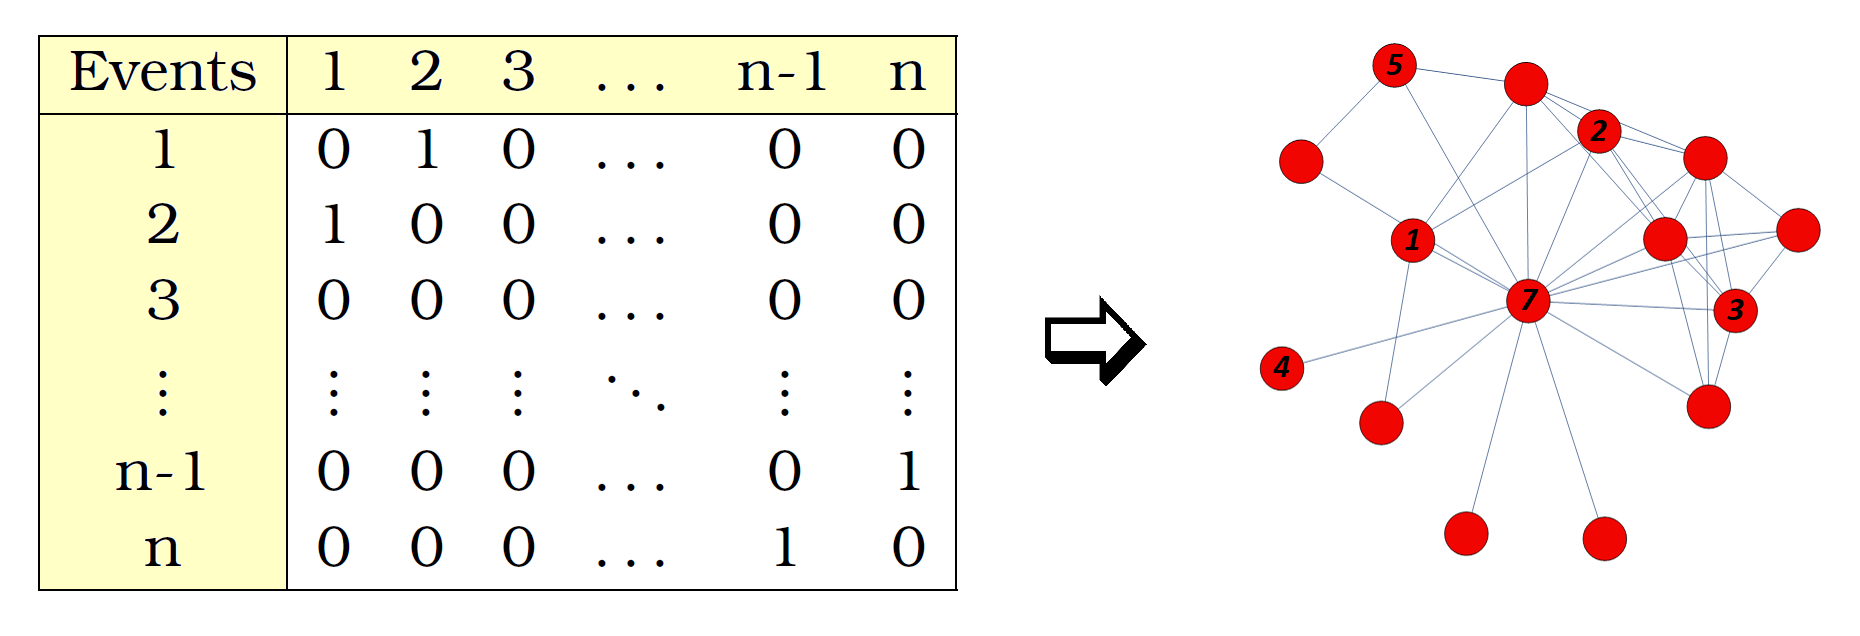
\includegraphics[width=0.7\linewidth]{../images/methodology-association-networks-adjacency_graph.png}}
		\caption{An Arbitrary Representation for Adjacency Matrix and Its Graph.}
		\label{figure-adjacency_graph}
	\end{center}
\end{figure}

%\begin{table}[]
%	\begin{tabular}{|c|cccccc|}
%		\hline
%		Events & 1   & 2   & 3   & \dots & n-1 & n   \\ \hline
%		1      & 0   & 1   & 0   & \dots & 0   & 0   \\
%		2      & 1   & 0   & 0   & \dots & 0   & 0   \\
%		3      & 0   & 0   & 0   & \dots & 0   & 0   \\
%		\vdots & \vdots & \vdots & \vdots & \ddots & \vdots & \vdots \\
%		n-1    & 0   & 0   & 0   & \dots & 0   & 1   \\
%		n      & 0   & 0   & 0   & \dots & 1   & 0   \\ \hline
%	\end{tabular}
%\end{table}
\subsection{Binning Schemes}\label{binning_schemes}
%\addcontentsline{toc}{subsection}{Binning Methods}%

The data set $D$ events can be labelled with a typical value interval (the so-called binning size) for the Feature-A values with a slight difference. Binning generation can be performed in alternative ways, allowing us to put the hypothetically created constraints into practice.

Say that we do the Feature-A values labelling with a typical binning size, in our case, 99, so that all of the events in $D$ must match the corresponding \ac{fss} interval, as shown in Table~\ref{Tab: D-dataset-FSS}. 
\begin{table}[ht!]
	\centering
	\setlength{\arrayrulewidth}{0.79pt}%
	\caption{Data Set D with FSS Bin Size Labels.} 
	\begin{tabular}{|cc|c|ccc|c|}
		\hline \rowcolor[HTML]{FFFFC7}
		\makecell{Event\\ID} 	&& Feature-A    	&& FSS Bins && \makecell{Sequence\\ID}  \\ \hline
		1 	      && 280	    && 200-299	&& 1 		     \\
		2 		  && 250	    && 200-299	&& 1 		     \\
		3 	      && 890	    && 800-899	&& 2 		     \\
		4 		  && 850	    && 800-899	&& 2 		     \\
		\vdots	  && \vdots  	&& \vdots	&& \vdots 	     \\
		n-2 	  && 520	    && 500-599	&& k 		     \\
		n-1       && 630	    && 600-699	&& k 		     \\
		n 		  && 610	    && 600-699	&& k 		     \\ \hline
	\end{tabular}
	\label{Tab: D-dataset-FSS}
\end{table}

An alternative way of label generation is to create bins with equal event counts per bin among the complete data set; \ac{fbs} labelling is shown in Table~\ref{Tab: D-dataset-FBS}.
\begin{table}[ht!]
	\centering
	\setlength{\arrayrulewidth}{0.75pt}%
	\caption{Data Set D with FBS Bin Size Labels.}
	\begin{tabular}{|cc|c|ccc|c|}
		\hline \rowcolor[HTML]{FFFFC7}
		\makecell{Event\\ID} 	&& Feature-A    	&& FBS Bins && \makecell{Sequence\\ID} \\ \hline
		1 	      && 280	    && 200-599	&& 1 		     \\
		2 		  && 250	    && 200-599	&& 1 		     \\
		3 	      && 890	    && 630-899	&& 2 		     \\
		4 		  && 850	    && 630-899	&& 2 		     \\
		\vdots	  && \vdots  	&& \vdots	&& \vdots 	     \\
		n-2 	  && 520	    && 200-599	&& k 		     \\
		n-1       && 630	    && 630-899	&& k 		     \\
		n 		  && 610	    && 600-629	&& k 		     \\ \hline
	\end{tabular}
	\label{Tab: D-dataset-FBS}
\end{table}
The alternative binning generation methods mentioned above let us derive two distinguished approaches to construct association networks. The first one is the \acs{fss} Network approach; it has graph nodes as binning groups with equal bin sizes. Manipulation of binning size allows us to aggregate events in different network nodes. The \acs{fbs} Network approach is the second one where the network nodes are binning groups with an equal number of events per bin. Defining a typical bucket size for the network nodes results in arbitrary interval boundaries for each node, and it allows to control their population.
 \begin{figure}[!ht]
	\begin{center}
		\makebox[\textwidth]{
			\centering
			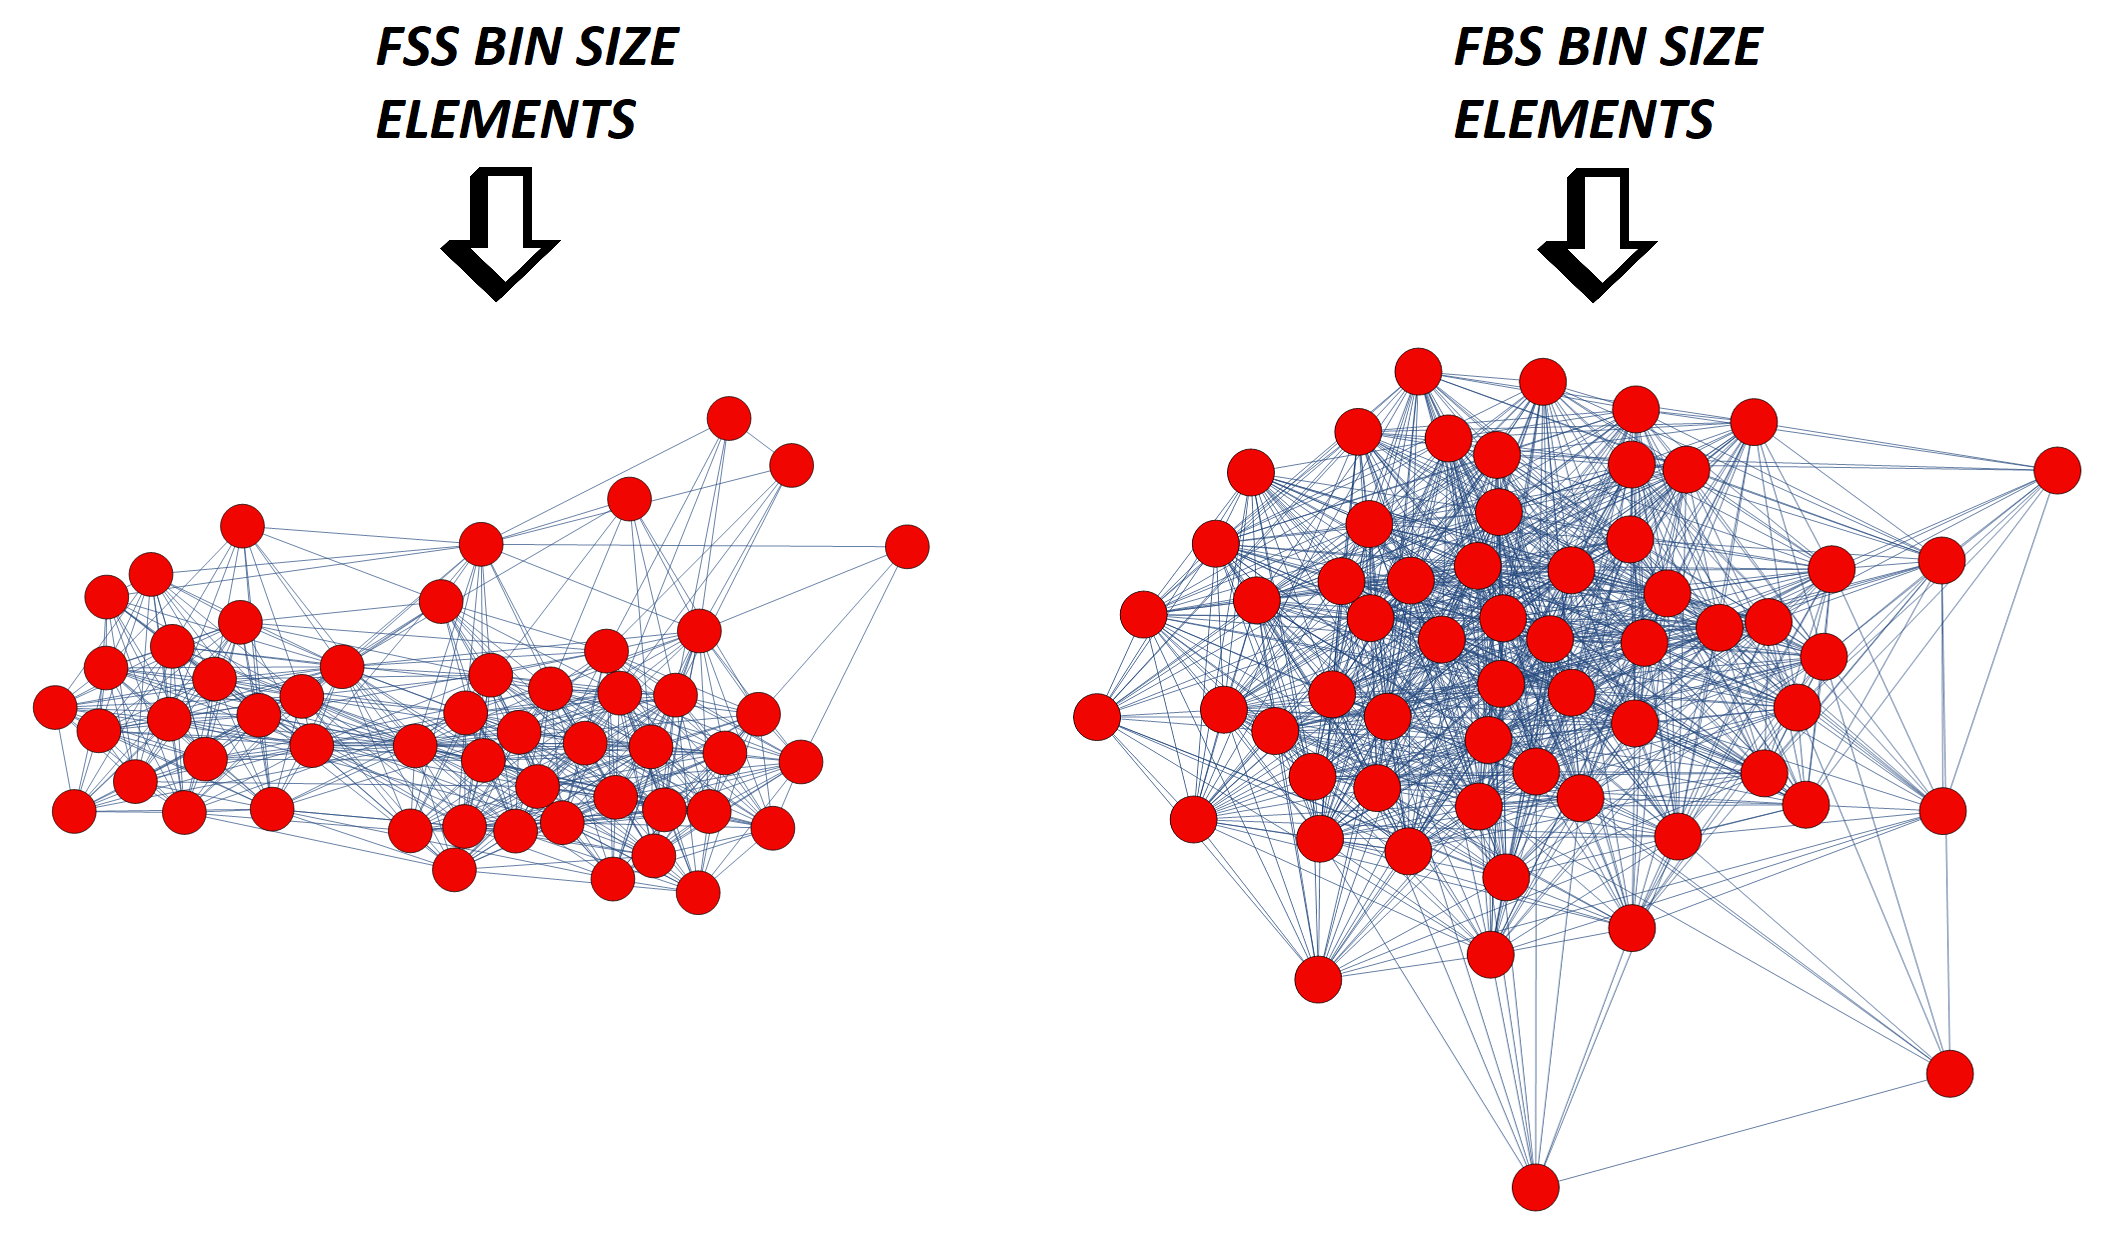
\includegraphics[width=0.8\linewidth]{../images/methodology-association-networks-hyp_networks.png}}
		\caption{Graph Results For Two Different Network Approaches.}
		\label{figure-hyp_graphs}
	\end{center}
\end{figure}

Constructing \acs{fss} and \acs{fbs} networks for the production events concerning technology-driven constraints and load-driven constraints underlie the developed hypothesis of this thesis work: Non-random features of the association networks derived from these two approaches.
\subsection*{Network Metrics Analysis}
\addcontentsline{toc}{subsection}{Network Metrics Analysis}%
\subsubsection*{Modularity}
As explained in the previous subsection, one data set can be labelled in alternative ways with FSS and FBS binning methods. Consecutively, nonsimilar network motifs will be obtained as output. That variety of textures emerge from the nodes having different degree values within their neighbourhood.

The degree is a network metric that quantifies one node's links to the other nodes~\cite{Barabasi2016}. It is a way to express the network characteristics. It gives us an idea about the connectivity patterns within the network and allows us to distinguish the group of nodes with a high degree from the nodes with a low degree. 

The nodes clustered together form significant communities or modules in the graph; those patterns give insight into how the data elements are related in the whole network. Modularity is a network measure for community detection and quantifies the strength of community structure in that specific network.

Newman (2006) formulated modularity in his article as
\begin{equation} \tag{1}
	Q = \frac {1} {2 m}\sum_ {ij} (A_{ij} - \frac {k_{i} k_{j}}{2 m}) \
	\frac {s_{i} s_{j} + 1} {2}\ ,
	\label{modularity}
\end{equation}
where the network has an $m$ number of edges, and $A_{ij}$ is the number of edges between vertices $i$ and $j$. $A_{ij}$ is the element of the adjacency matrix introduced in Fig.~\ref{figure-adjacency_graph}. It can be $0$ or $1$. $k_{i}$, and $k_{j}$ are the vertex degrees, and ${k_{i} k_{j}}/{2 m}$ is the expected number of edges between $i$ and $j$ if edges are placed at random. $s_{i}$ and $s_{j}$ are the divided network groups. They are equal to $1$ if $i$ and $j$ belong to the same group and $0$ otherwise. Eq.\eqref{modularity} is used to divide the network into two communities only; however, many networks may contain more than two communities. Therefore, a repeated division into two is adapted: dividing the network into two graphs, then the two sub-graphs further divided into two only if that would maximize $Q$. After first partitioning, the edges falling between the further divided sub-graphs are neglected, leading to the wrong maximization quantity. For this reason, the author introduced the additional contribution $\Delta Q$.~\cite{Newman8577}
% $B_{ij} = A_{ij} - \frac {k_ {i} k_ {j}} {2 m}$\\
% $Q = \frac {1} {4 m} s^{T} Bs = \frac {1} {4 m}\sum_ {i = 
%	1}^{n} (u_ {i}^{T} . s)^{2}\beta_ {i}$\\
% $\Delta Q = \frac {1} {4 m} s^{T} B^{(g)} s$\\
% $B_{ij}^{(g)} = B_{ij} - \delta_{ij}\sum_ {k\in g} B_{ik}$

Since the results obtained with the combination of $Q$ and $\Delta Q$ do not significantly differ from the results obtained only using $Q$, modularity calculations in this work were performed with the latter to lower the computation timing.
\clearpage

\subsubsection*{Different Types of Null Model}
{\color{red} If I have more than two modules, do I conserve the specific number of inter-module edges per module pair? Would a link between module 1 and 2 be shuffled with a link between modules 1 and 3? 
	All the interlinks independent from the number of modules are shuffled in the same set. I did not consider different module interlinks in separate groups. It is a design decision.
	
	In particular, if I do not have the pleasant situation that people usually think of in a modular graph where the connectivity between modules is typically about the same for any pair of modules. But if I have a slightly more realistic situation where module pairs differ very strongly in the way they are interconnected. In real-life data, I often have two challenging modules to separate because they are tightly interconnected and then maybe one or two other modules that are almost not connected to the other modules. That is the part that I do not conserve and might affect the result.
	
	Fixed Degree Sequence random graphs generation, a third one: Conserving Inter-edges and Intra-edges Among Modules random graphs were generated; accordingly, Z-scores were computed among those null models.
	
	I have recomputed my constraint impact analysis pipeline for four production lines with null models: Degrees Fixed and Modularity and different choice of binning in terms of step-size \& bucket-size.
	
	Since plot results vary based on a specific randomization null model, discussing how shuffling was performed is essential. 
	Random graphs were generated, and the below instruments were plotted.
	Modularity vs time windows
	Average modularity for single random graph vs time windows
	Z-scores for modularity randomized null models with modularity conserved vs time windows
	Z-scores for modularity randomized null models with fixed degree sequences vs time windows
	
	
	The cartoon showing how I generated the null models in a pairwise shuffling fashion to prevent ambiguity.}

 \begin{figure}[!ht]
	\begin{center}
		\makebox[\textwidth]{
			\centering
			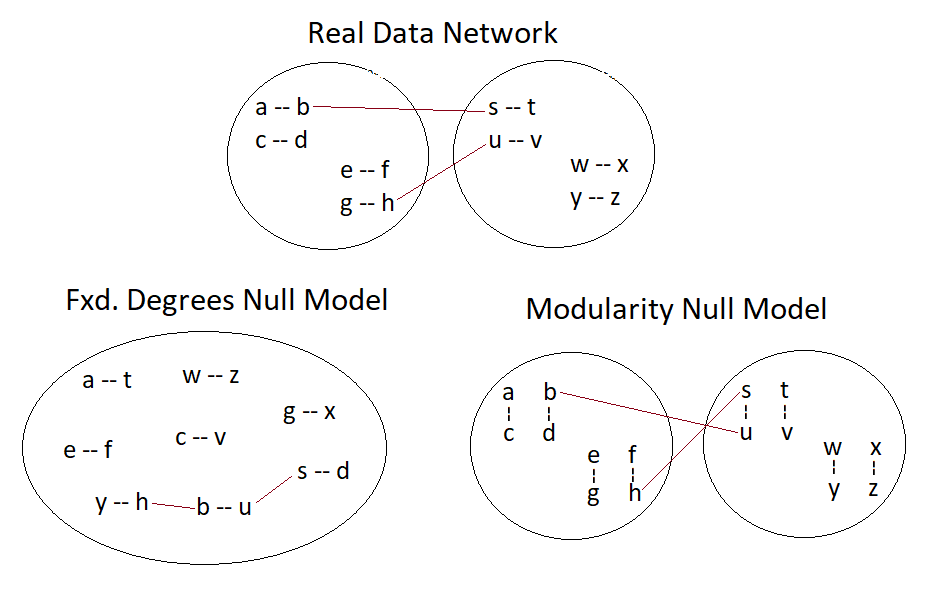
\includegraphics[width=0.6\linewidth]{../images/cartoon-null-model-definitions.png}}
		\caption{Formation of Different Null Models.}
		\label{figure-null_models}
	\end{center}
\end{figure}

{\color{red}
	Introduce hierarchical modularity and its relation with null models.
	
	The full z-score curves are only there because we want to ensure that we don't overlook something. If the full curves are drastically away from zero, then the type of modularity in the real graphs are somewhat different. They are either very asymmetric with respect to the modules or hierarchical or anything else that is very complicated. In some sense, the full curves are just a reference check to whether everything works as expected and whether it is meaningful to discuss modularity. So what we are really looking at is the dashed curves. And I am looking at the z-score only; I am trying to figure out whether the step from FSS to FBS drastically changes the modularity. I am wondering whether we can condense this further to make this information is more accessible.
	
	If the full z-score curves are always close to zero for both different network approaches, would that give us an idea about the modularity? Then it says that the modularity is as we expect the modularity to be. 
	
	If I have a very modular graph and then I randomize it such that I conserve the modularity. Then the comparison of the original modular graph with the randomized modular graphs will lead me to a zero z-score, no matter what the modularity is. 
	
	The dashed line is the more meaningful null model, but we need the other null model because modularity might have strange effects. For example, if the real network has a hierarchical structure, modules within modules within modules, I would still see modularity (positive z-score with respect to the null model behind the full curve) because I am destroying the other type of modularity (nested modularity) in my null model. So in some sense, this is just checking that we have that type of (nested) modularity in deep.
	
	If you have a strongly modular network and each module is in itself modular, then in my null model that preserves modularity, I would destroy that internal modularity of modules. So I would have positive z-scores (full lines would be shifted upwards).
	
	If the full curves are positive, it means we have modules in modules. If the full curves are negative, it means (guessing a bit) that we have big differences in the number of inter-module links. So that some modules are tightly connected while other modules are sparsely connected. And in my null model, this is average. That means that the modularity in the randomized module-conserving networks is actually higher.
	
	Is the dashed curve of FSS higher than the dashed curve of FBS? That's a type of information we should extract from those plots/bar charts.
	
	Performing switch-randomization to a modular graph might fail even due to small details in randomization steps. That failure is probably the reason for the high values of Z-scores in two different plots of Z-scores. If I try to switch-randomize a modular graph, I could imagine a procedure where I take links only from the same module and switch them or links across modules and switch them. And I mixed the sets of intra-module edges and inter-module edges separately. This null model might give a different result in Z-scores.}
\clearpage
\section{Simulation Model}
The genome-scale integrated networks are necessary tools used by metabolic engineers on model design, theoretical and computational analysis to understand how the biological system of microbial organisms works~\cite{HAO}. In addition, integrated network theory tools expand the feasible space for analysis techniques in further work steps. As an initial step, one can construct a network showing interactions between metabolites, intermediate or end products and metabolic reactions for an organism. 

The set of rules for the organism can be represented in a compact form by an m-by-r matrix formulation as
\begin{equation} %\tag{1}
	S =  \begin{bmatrix} 
		s_{11} & s_{12} & \dots  & s_{1r}\\
		s_{21} & s_{22} & \dots  & s_{2r}\\
		\vdots & \vdots &\ddots & \vdots \\
		s_{m1} & s_{m2} & \dots & s_{mr} 
	\end{bmatrix}=(s_{ij})\in \mathbb{Z}^{mxr}.
	\label{stoichio}
\end{equation}
\myequations{Stoichiometric Matrix}
The matrix $S$ is called stoichiometric matrix, its column elements represent reactions that play a role in the chemical transformations, and its row elements represent metabolites. $S$ also contains direction information for the related metabolite-reaction element in the matrix with positive or negative signs.~\cite{klipp2005systems} 

Having transpose of $S$ will reverse the columns and rows in the matrix as 
\begin{equation}
	S^{T} =  \begin{bmatrix} 
		s_{11} & s_{12} & \dots  & s_{1m}\\
		s_{21} & s_{22} & \dots  & s_{2m}\\
		\vdots & \vdots &\ddots & \vdots \\
		s_{r1} & s_{r2} & \dots & s_{rm} 
	\end{bmatrix};
	\notag
\end{equation}
thus, by the product of $S$ and $S^{T}$, we obtain two different matrices as

\noindent\begin{minipage}{.5\linewidth}
	\begin{equation}
		S.S^{T} =  \begin{bmatrix}
			s^{'}_{11} & s^{'}_{12} & \dots  & s^{'}_{1m}\\
			s^{'}_{21} & s^{'}_{22} & \dots  & s^{'}_{2m}\\
			\vdots & \vdots &\ddots & \vdots \\
			s^{'}_{m1} & s^{'}_{m2} & \dots & s^{'}_{mm} 
		\end{bmatrix}
		\notag
	\end{equation}
\end{minipage} and
\begin{minipage}{.5\linewidth}
	\begin{equation}
		S^{T}.S =  \begin{bmatrix}
			s^{''}_{11} & s^{''}_{12} & \dots  & s^{''}_{1r}\\
			s^{''}_{21} & s^{''}_{22} & \dots  & s^{''}_{2r}\\
			\vdots & \vdots &\ddots & \vdots \\
			s^{''}_{r1} & s^{''}_{r2} & \dots & s^{''}_{rr} 
		\end{bmatrix},
		\notag
	\end{equation}
\end{minipage}

where $S.S^{T}$ is a metabolite-centric matrix and $S^{T}.S$ is a reaction-centric matrix. Considering a normalising step for those matrices as 
\begin{equation}
	f(x) =
	\begin{cases}
		0, & \text{if}\ x = 0 \\
		1, & \text{if}\ x \neq 0
	\end{cases},
	\notag
\end{equation}
one can construct adjacency matrices, $A^{m}_{ij}=f(s^{'}_{ij})$ and $A^{r}_{ij}=f(s^{''}_{ij})$, to form graphs like that introduced in Fig.~\ref{figure-adjacency_graph} in the Association Networks subsection. 

The graphs in Fig.~\ref{figure-metabolic-networks} were generated from $A^{m}$ and $A^{r}$ using a stoichiometric matrix belonging to homo sapiens metabolism retrieved from BiGG Models Database~\cite{biggmodels}. In Fig.~\ref{figure-metabolic-centric}, the graph nodes stand for the metabolites, and graph edges are the reactions. In contrast, in Fig.~\ref{figure-reaction-centric}, the roles are reversed so that the graph edges represent the metabolites, and the graph nodes represent the reactions.
\begin{figure}[!ht]
	\centering
	\begin{subfigure}{0.5\textwidth}
		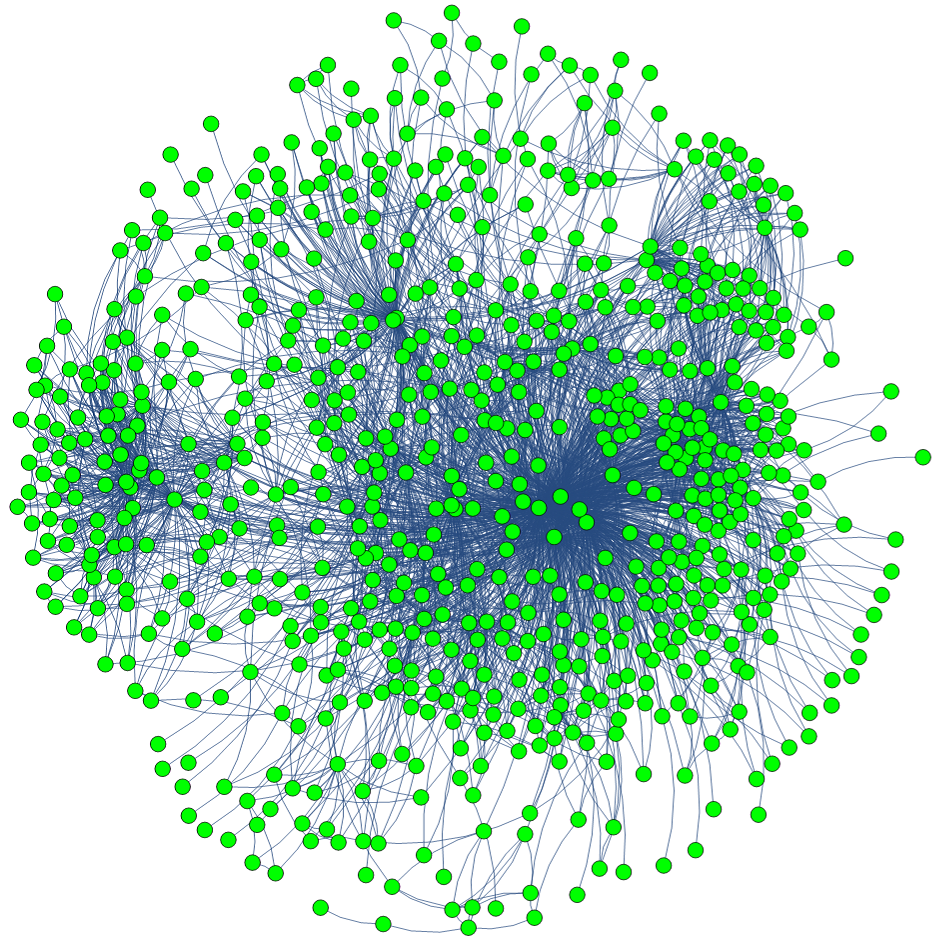
\includegraphics[width=1\linewidth]{../images/methodology-ORmodel-metabolic_centric_network.png}
		\caption{Metabolic-centric Network}
		\label{figure-metabolic-centric}
	\end{subfigure}\hfill% or \hspace{5mm} or  \hspace{0.3\textwidth}
	\begin{subfigure}{0.5\textwidth}
		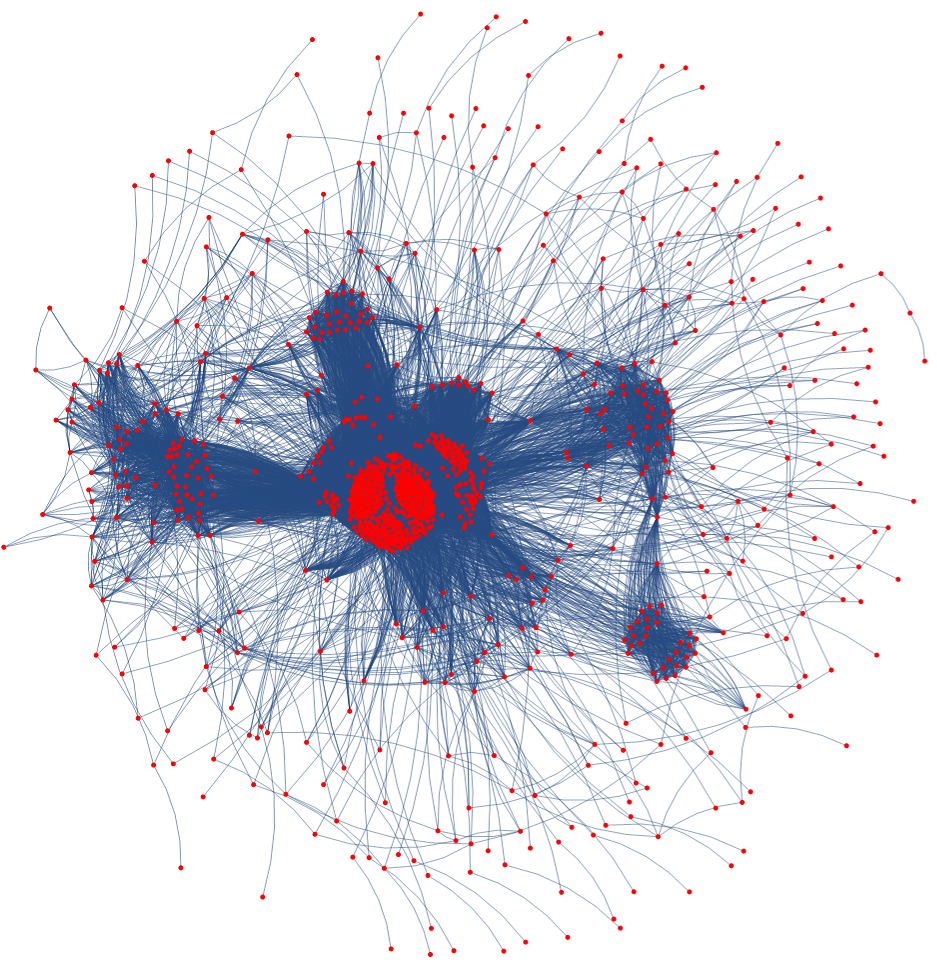
\includegraphics[width=1\linewidth]{../images/methodology-ORmodel-reaction_centric_network.png}
		\caption{Reaction-centric Network}
		\label{figure-reaction-centric}
	\end{subfigure}
	\caption{Network Representations for Homo Sapiens Metabolic Model}
	\label{figure-metabolic-networks}
\end{figure}

Studying biological metabolic systems and designed models to achieve cellular objectives like cell growth or ATP (Adenosine Triphosphate Production) necessitates various tools to be integrated with reconstructed genome-scale networks~\cite{KIM, HAO}. One of the commonly used tools is Flux Balance Analysis (FBA) as an optimization scheme. It is a constraint-based modelling approach to simulate microbial metabolisms and can be applied to biochemical-reaction networks containing the chemical transformations and flux exchanges~\cite{KAUFFMAN2003491, PRICE2004}.

While one can express the metabolic fluxes in a one-dimensional array (the so-called flux vector $V$) as
\begin{equation} %\tag{2}
	V = \begin{bmatrix}
		v_{1} \\
		v_{2} \\
		\vdots \\
		v_{r}
	\end{bmatrix}=(v_{i})\in \mathbb{R}.
	\label{solutionvector}
\end{equation}
\myequations{Fluxes Solution Vector}
$V$ contains flux exchange values for the corresponding reactions in the system and gives information about the flux distribution; hence, those can be both positive and negative real numbers. Defining a mass-balance ($S.V=0$) constraint in the FBA enables us to analyze the metabolic network operations in a steady-state solution space~\cite{KAUFFMAN2003491,PRICE2004}.
\begin{equation} %\tag{3}
	S.V = \begin{bmatrix} 
		s_{11}v_{1} + s_{12}v_{2} + \dots + s_{1r}v_{r} \\
		s_{21}v_{1} + s_{22}v_{2} + \dots + s_{2r}v_{r} \\
		\vdots \\
		s_{m1}v_{1} + s_{m2}v_{2} + \dots + s_{mr}v_{r} 
	\end{bmatrix}=
	\begin{bmatrix} 
		0 \\
		0 \\
		\vdots \\
		0
	\end{bmatrix}.
	\label{massbalanceconstraint}
\end{equation}
\myequations{Mass Balance in Steady State}
The higher amount of metabolite consideration in the set of rules, $S$, in other words, the larger matrix size by its rows amount means the more complex type of organization structure taken into account while preserving the steady-state in the whole system.

More than one steady-state solution might be present since it is impossible to identify all constraints in a cellular system~\cite{KAUFFMAN2003491}. Therefore, one can formulate an optimization approach to identify reaction network steady-states that maximize the biomass~\cite{KAUFFMAN2003491,PRICE2004} or control the production of specific metabolites~\cite{VARMA1993} within a defined objective function under the consideration of the system constraints. According to Price et al. (2004),
there are three primary purposes to generate objective functions~\cite{PRICE2004}:
\begin{itemize}
	\item[i.] to discover allowable characteristic properties in the genome-scale network reconstruction,
	\item[ii.] to mimic probable physiological functions like biomass or ATP production to be able to determine likely physiological states and
	\item[iii.] to design a genetic variant or sub-type to obtain a desired particular product.
\end{itemize}

One can express objective function coefficients in a one-dimensional array as
\begin{equation} %\tag{4}
	O =  \begin{bmatrix}
		o_{1} & o_{2} & \dots  & o_{r}\\
	\end{bmatrix}=(o_{i})\in \mathbb{R}.
	\label{objectivecoefficients}
\end{equation}
\myequations{Objective Function Coefficients Array}
As given in Eq.~\eqref{biomassmaximisation}, the biomass formulation delivers the output with its non-zero coefficients, which are the decisive ones for the flux elements of $V$ to be considered.
\begin{equation} %\tag{5}
	O.V = (o_{1}v_{1} + o_{2}v_{2} + \dots + o_{r}v_{r})\in \mathbb{R}_{\ge0}.
	\label{biomassmaximisation}
\end{equation}
\myequations{Maximized Biomass}
Stoichiometric (or mass-balance) constraints were introduced so far in Eq.~\eqref{stoichio} and Eq.~\eqref{massbalanceconstraint}. In addition, upper and lower bounds are presented for particular fluxes in $V$ during the optimization process. The bounds are used in the reactions for uptake and secretion of any organic metabolite. In the uptake reactions, nutrients are transported to the inside of the metabolic network. In the secretion reactions, products are exported to the outside of the network. The rest of the fluxes in $V$ are used in the exchange reactions, namely the intermediate reactions in the network. The constraints influence the reactions for uptake and secretion, whereas no limitation is considered in the exchange reactions. Quantifying imported nutrients and exported outputs (resources and products) by constraining them with upper and lower bounds to fulfil a single objective function goal might significantly influence the optimization process.

 \begin{figure}[!ht]
	\begin{center}
		\makebox[\textwidth]{
			\centering
			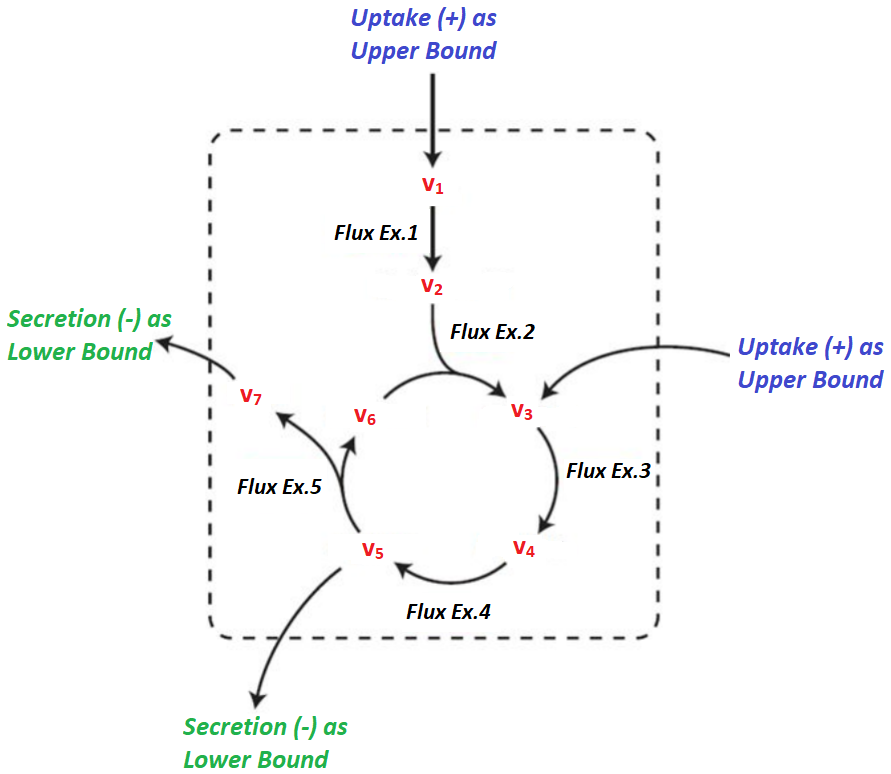
\includegraphics[width=0.57\linewidth]{../images/methodology-ORmodel-uptake_secretion_cartoon.png}}
		\caption{A Simplified Reaction-centric Network Sketch Shows The Reactions for Exchange, Uptake and Secretion.}
		\label{figure-uptake-secretion-cartoon}
	\end{center}
\end{figure}

As a summary of the above-explained series of constraints, mass-balance equality (Eq.~\eqref{massbalanceconstraint}), upper \& lower bounds for fluxes (Fig.~\ref{figure-uptake-secretion-cartoon}), and the objective function (Eq.~\eqref{objectivecoefficients}) are the three fundamental constraints that set off a linear programming problem because it is possible to formulate them linearly~\cite{PRICE2004}. The optimization result: flux vector $V$ (Eq.~\eqref{solutionvector}) maximizes the objective function in the form of a flux distribution~\cite{KAUFFMAN2003491,PRICE2004}. Since each term in Eq.~\eqref{biomassmaximisation} is a produced biomass expression for the fluxes, the summation of those terms will give the overall growth of the system for a single network state.

Different solution vectors of $V$ can be obtained from the linear optimization process by varying the constraints introduced above. As a compact set of rules, the stoichiometric constraints significantly influence the mass-balance equation; consequently, the solution vector $V$~\cite{Edwards2001}. A stoichiometric matrix from scratch can be formulated, ensuring the mass-balance constraints are incorporated in the reaction cycles of the investigated system. However, the homo sapiens metabolic model was taken as the set of rules in this thesis work. Varying upper \& lower flux bounds and the objective function are the two alternative approaches introduced in the following subsections to understand the model behaviour while the optimization is carried on.
\subsection*{Resource Utilization}
\addcontentsline{toc}{subsection}{Resource Utilization}%
Environmental conditions such as resource availability affect the pattern of outputs in a metabolic network. In case of fewer resources (nutrients) availability, the active production network gets more interconnected through more flux exchanges to produce the necessary input for the ongoing metabolic reactions.~\cite{PRICE2004,MAHADEVAN2003,Reed01092004,BURGARD2001}
\begin{equation} %\tag{6}
	V^{b}=\{v^{b}_{1}, v^{b}_{2},\dots, v^{b}_{x}\}= (-a\le v^{b}_{i}\le a)\in V
	\label{constrainedfluxlist}
\end{equation}
\myequations{Constrained Fluxes List}
Let $V^{b}$ is a list of fluxes with $x$ elements randomly picked from $V$ (Eq.~\eqref{solutionvector}) to be limited with the bounds: $(-a, a)$. The same tolerance in both negative and positive direction for the bounds allows the network to treat the respective flux flow as uptake or secretion based on the system need. The fluxes that are not included in $V^{b}$ are matched with extreme high boundary values so that they are not constrained while the linear optimization.
\begin{equation} %\tag{7}
	V^{e}=\{v^{e}_{1}, v^{e}_{2},\dots, v^{e}_{y}\}= (0\le v^{e}_{i}\le 0)\in V
	\label{deletedreactions}
\end{equation}
\myequations{Deleted Fluxes List}
Assigning zero to the upper \& lower bounds suppresses the respective flux exchange in the active production network. Those fluxes can not be used for the uptake, secretion, nor intermediate reactions. $V^{e}$ (Eq.~\eqref{deletedreactions}) is the list of fluxes with $y$ elements randomly selected from $V$ (Eq.~\eqref{solutionvector}) to be deleted from the network by assigning zero to the bounds.

Such limitations on resources serve as capacity constraints defining the active reactions and reversibility of flux exchanges~\cite{Edwards2001}. Varying $x$ and $a$ in Eq.~\eqref{deletedreactions}, and $y$ in Eq.~\eqref{deletedreactions}, we obtain various biomass values by the linear programming algorithm to fulfil a fixed objective function.

\subsection*{Production Portfolio Diversification}
\addcontentsline{toc}{subsection}{Production Portfolio Diversification}%
The objective function can be assumed as a production plan that rules the diversity of products that metabolism takes into account to maximize cellular growth~\cite{Edwards2001}. As previously mentioned, this is because the pattern of output biomass (Eq.~\eqref{biomassmaximisation}) is governed by the objective function (Eq.~\eqref{objectivecoefficients}). Its non-zero coefficients force the network for an optimal solution with their value range and positive and negative signs.    

Defining various arrays of objective function coefficients, consisting of elements with negative or positive signs, will allow us to create a diverse group of products that the network is capable of producing. In the same direction, adjusting the number of objective function terms is the second step of that diversification approach.
